\documentclass[a4paper]{article}
\usepackage{amsmath,amssymb,caption,enumitem,float,geometry,graphicx,indentfirst,minted,parskip,tabularx,xcolor}
\captionsetup[figure]{labelsep=period}
\captionsetup[listing]{labelsep=period}
\definecolor{bg}{rgb}{0.95,0.95,0.95}
\geometry{left=3.5cm,right=3.5cm,top=3.3cm,bottom=3.3cm}
\setlength{\parindent}{2em}
\usemintedstyle{emacs}
\begin{document}
\begin{titlepage}
    \vspace*{0.25cm}
    \noindent\rule[0.25\baselineskip]{\textwidth}{1pt}
    \begin{center}
        \huge{\textsc{UM--SJTU Joint Institute}}\vspace{0.3em}\\
        \huge{\textbf{System-on-Chip Design (ECE4810J)}}\vspace{0.3em}\\
        \noindent\rule[0.25\baselineskip]{\textwidth}{1pt}
    \end{center}
    \begin{center}
        \vspace{5cm}
        \Large{\textsc{Laboratory Report}}\vspace{0.5em}\\
        \Large{\textbf{Lab 2. Design with high level languages on Arty Z7 SoC development platform}}\vspace{1em}\\
        \Large{\textbf{Group 2}}\\
    \end{center}
    \vfill
    \large
    \begin{tabular}{ll}
        Name: Haochen Wu \hspace*{2em}&ID: 518021910558\hspace*{2em}\\
        Name: Yihua Liu \hspace*{2em}&ID: 518021910998\hspace*{2em}\\
        Name: Siyuan Zhang \hspace*{2em}&ID:
        518370910180 \hspace*{2em}\\
        \\
        Date: \today
    \end{tabular}
\end{titlepage}
\tableofcontents
\newpage
\section{Overview}
In this lab, we will go through two exercises to create design with high level languages (instead of Verilog). The goals of this lab are to:
\begin{itemize}
    \item Get familiar with the concept of High-level Synthesis (HLS)
    \item Learn to use HLS to create an IP block in C/C++
    \item Learn about differences between programming with HLS vs. Verilog in terms of design quality
    \item Get started with the Arty Z-7 board as a Python accelerator and be able to run example Jupyter notebook with the board
\end{itemize}
\section{Creating and using custom IP blocks using High-Level Synthesis}
\begin{figure}[H]
    \centering
    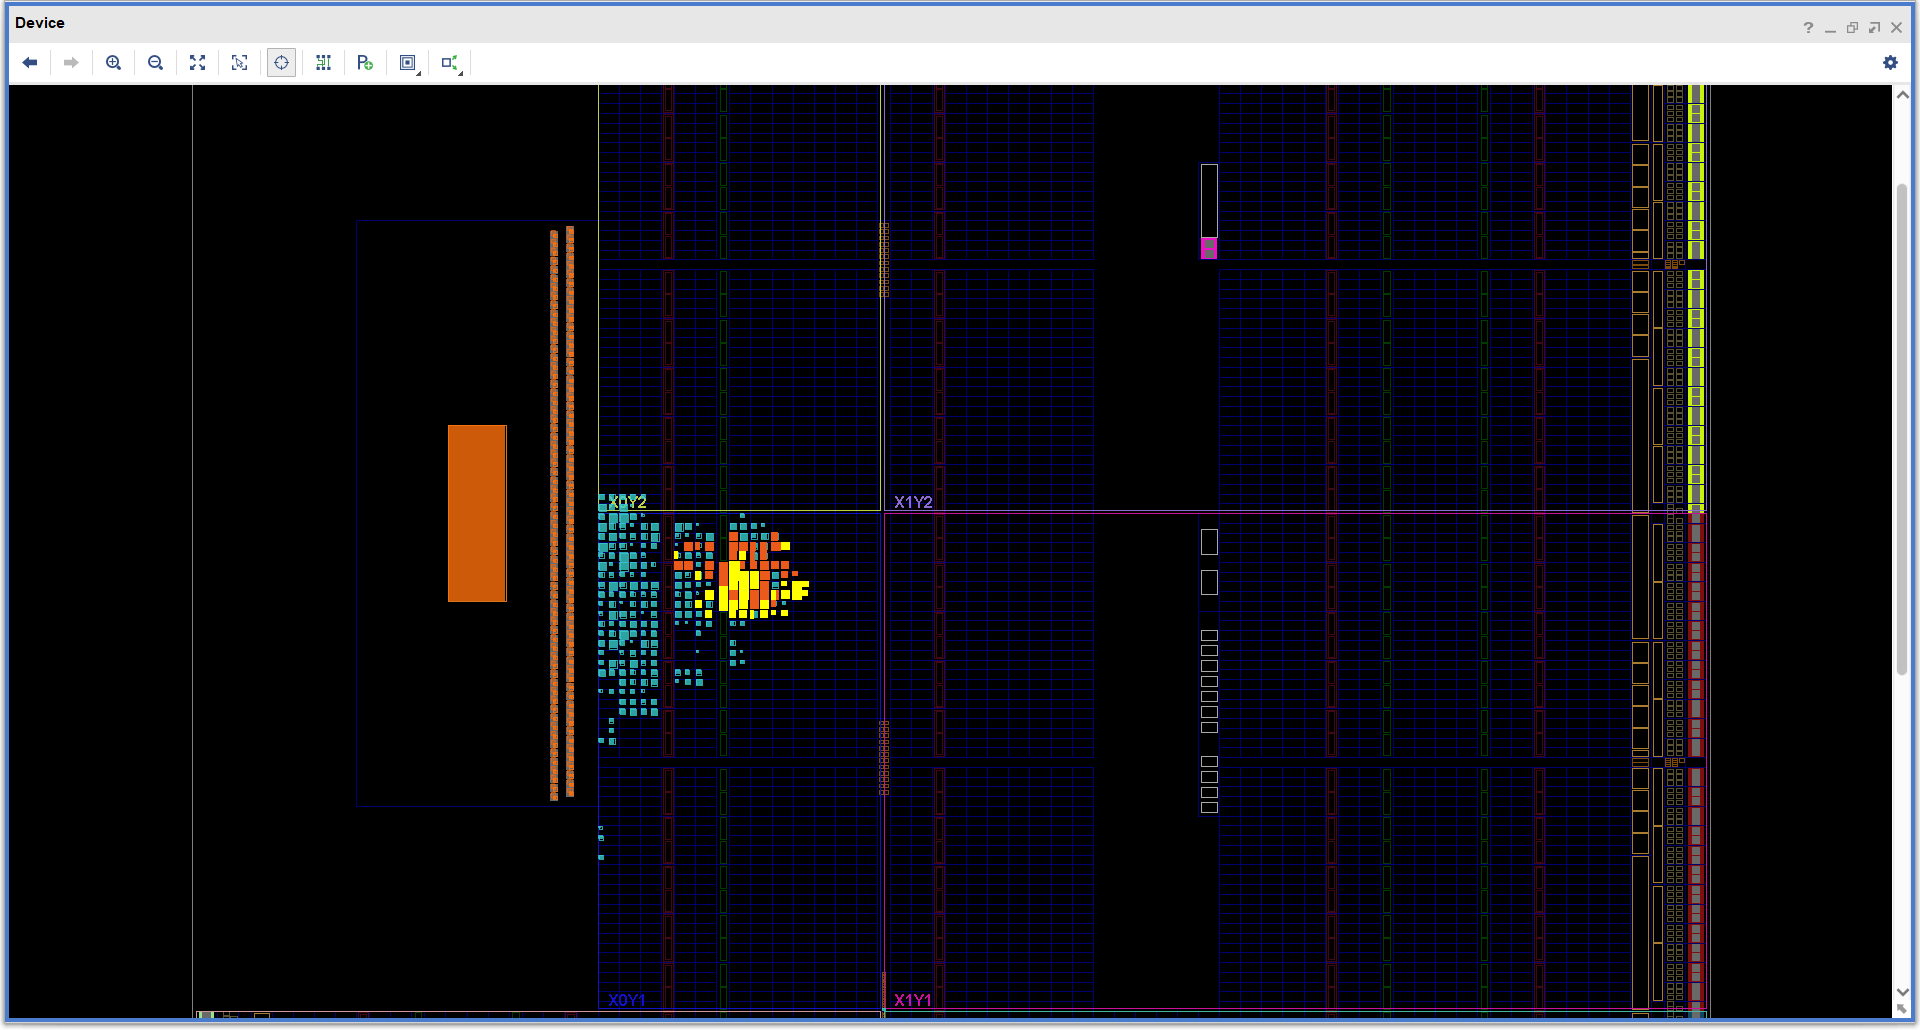
\includegraphics[width=1\textwidth]{1.png}
    \caption{The resource utilization of the HLS multiplier (screenshot).}
\end{figure}
The red leaf cells are RTL multiplier, and the yellow leaf cells are HLS multiplier. By comparing their area, we can find that the RTL implementation costs less resources, probably due to RTL version is more logically optimized and compact. 
\begin{figure}[H]
    \centering
    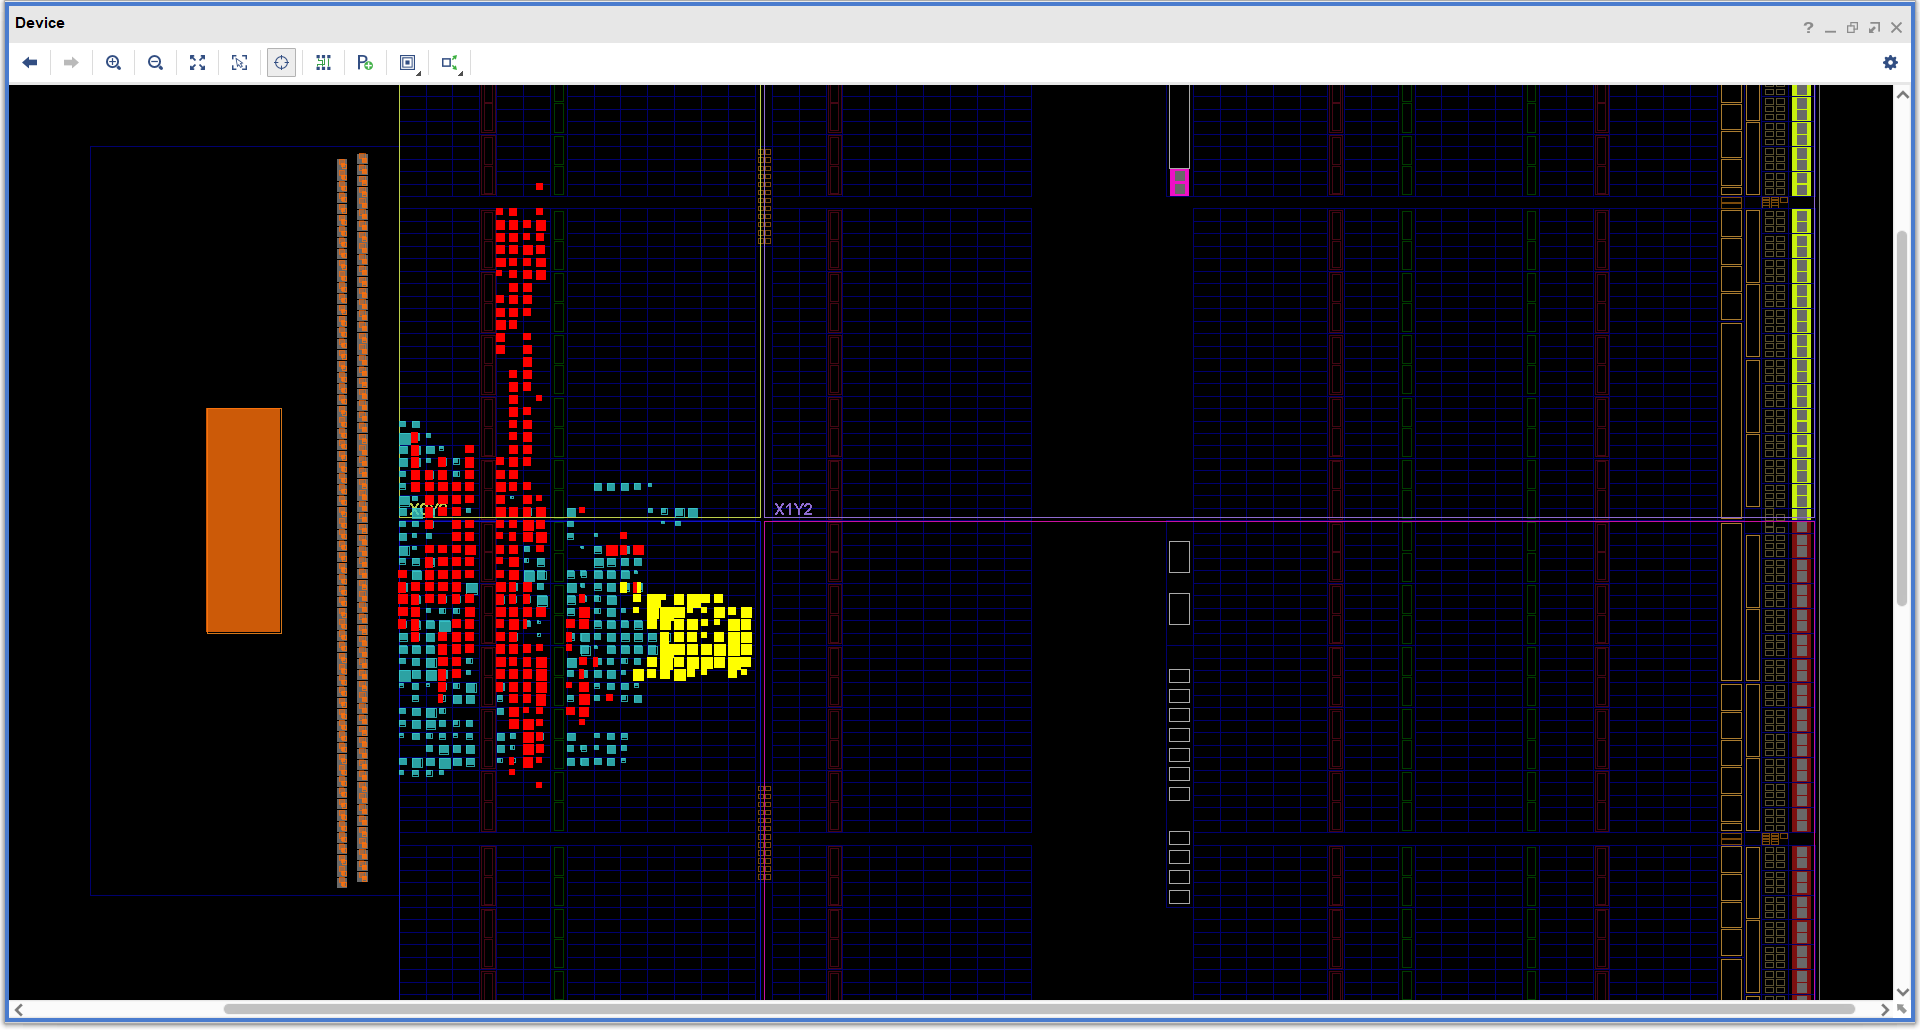
\includegraphics[width=1\textwidth]{2.png}
    \caption{The resource utilization of the HLS divider (screenshot).}
\end{figure}
For resource utilization of divider, the HLS consumes less area than RTL version. It's probably because RTL divider we write is not quite efficient, which costs so many resource usage.
\begin{listing}[H]
\inputminted[frame=single,bgcolor=bg,breaklines,linenos]{cpp}{test_hls_divider.cpp}
\caption{Source code of the resource utilization of the HLS divider (test bench).}
\end{listing}
\begin{listing}[H]
\inputminted[frame=single,bgcolor=bg,breaklines,linenos]{cpp}{hls_divider.cpp}
\caption{Source code of the resource utilization of the HLS divider (source).}
\end{listing}
\begin{figure}[H]
    \centering
    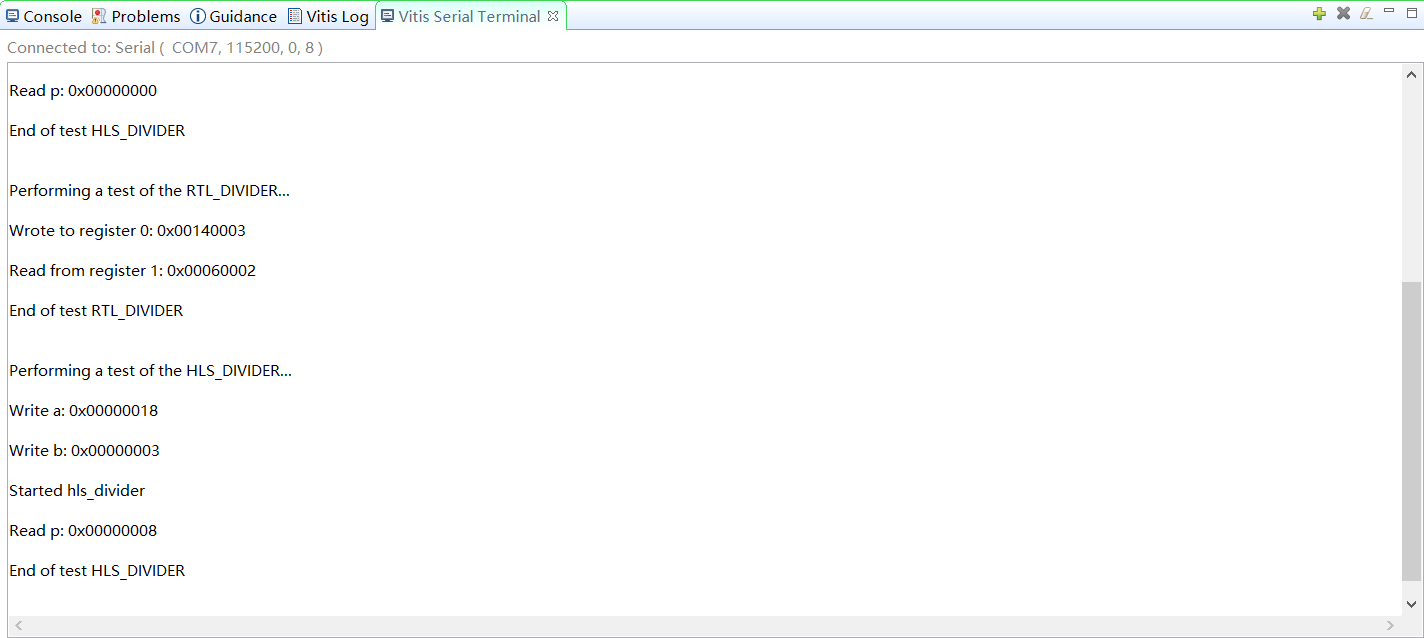
\includegraphics[width=1\textwidth]{3.png}
    \caption{SDK terminal printout of the HLS divider.}
\end{figure}
For RTL divider, we concatenate the quotient and the remainder together to form a 32-bit number to read from register 1. Since 20/3=6......2, the RTL can be verified as working properly. For HLS divider, we don't pertain this design, where the result is merely the qoutient, so 24/3=8.
\begin{listing}[H]
\inputminted[frame=single,bgcolor=bg,breaklines,linenos]{cpp}{hls_ALU.cpp}
\caption{Source code of ALU.}
\end{listing}
\begin{figure}[H]
    \centering
    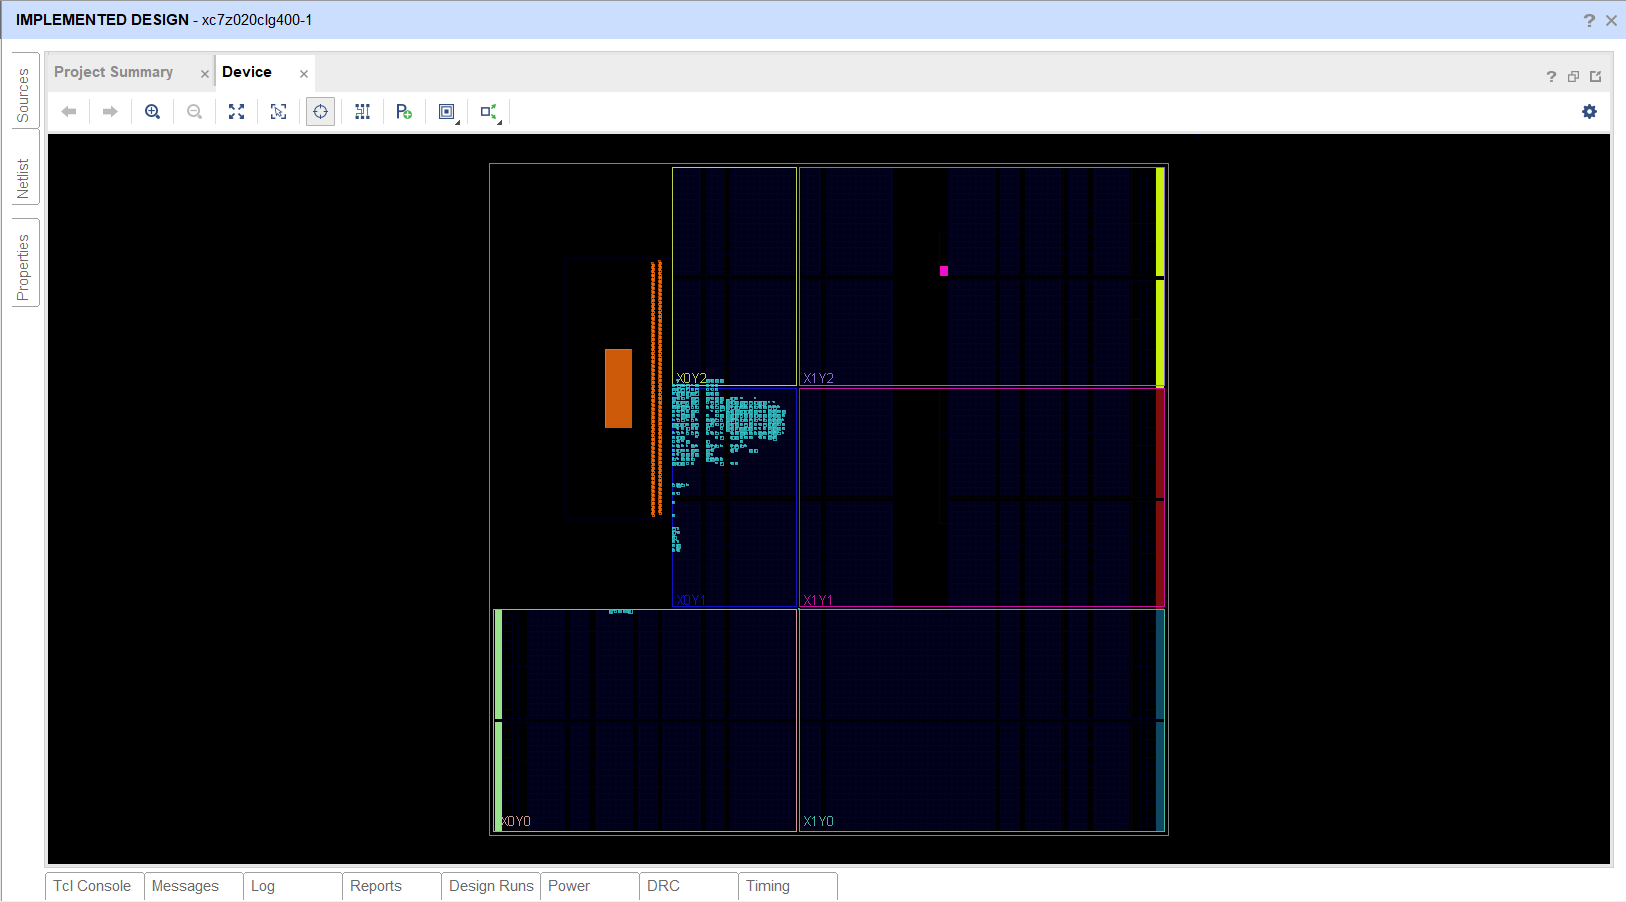
\includegraphics[width=1\textwidth]{4.png}
    \caption{The resource utilization of ALU.}
\end{figure}
\begin{figure}[H]
    \centering
    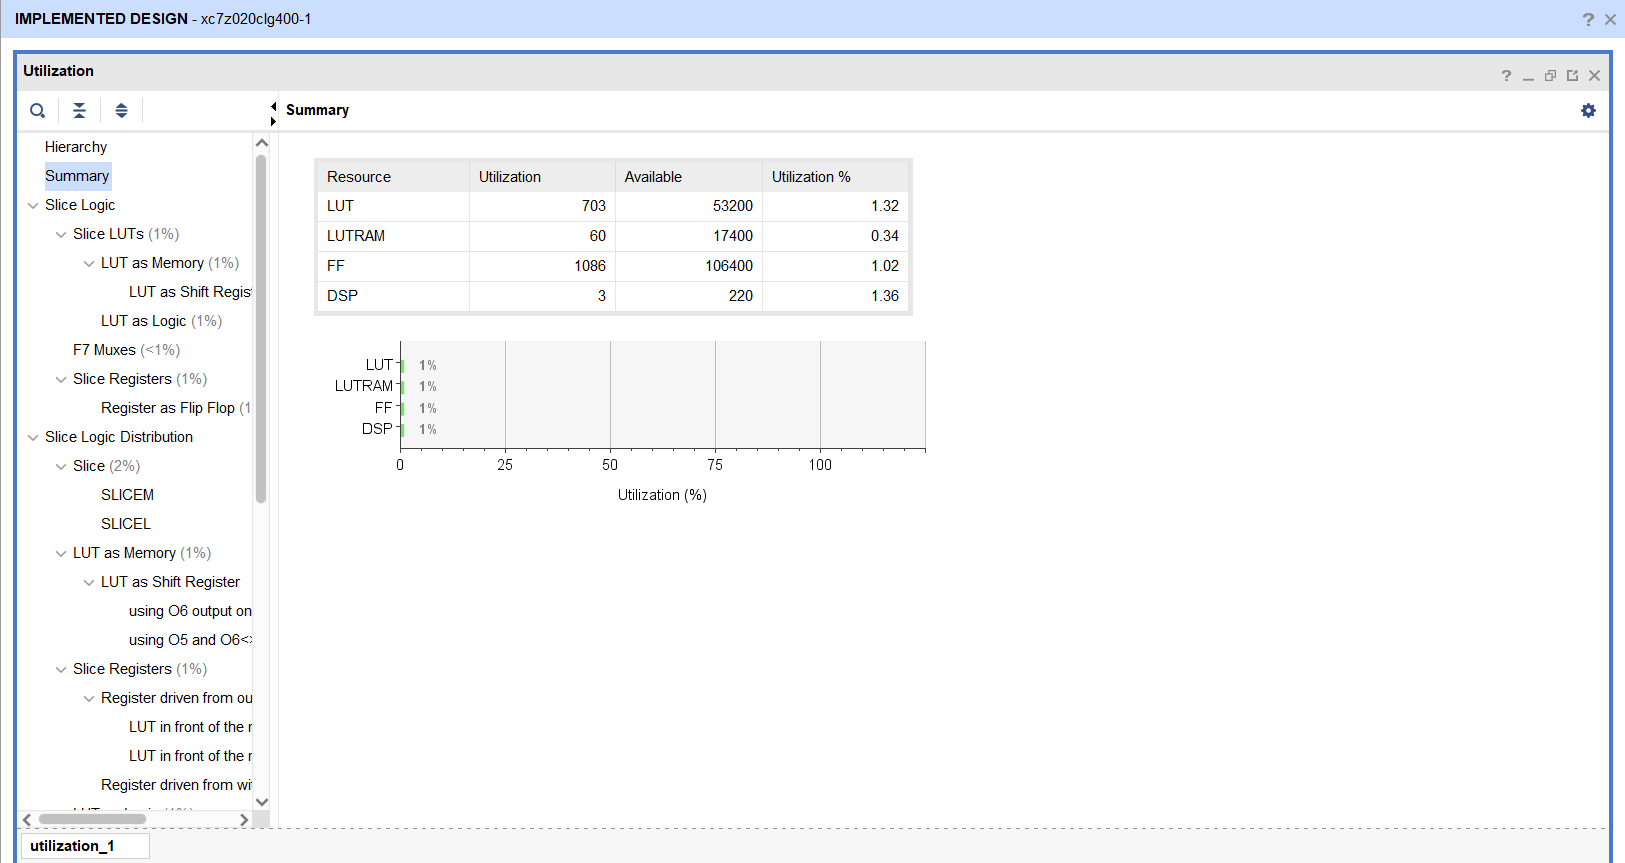
\includegraphics[width=1\textwidth]{5.png}
    \caption{The resource utilization of ALU (summary).}
\end{figure}
\begin{figure}[H]
    \centering
    
\includegraphics[width=1\textwidth]{6.png}
    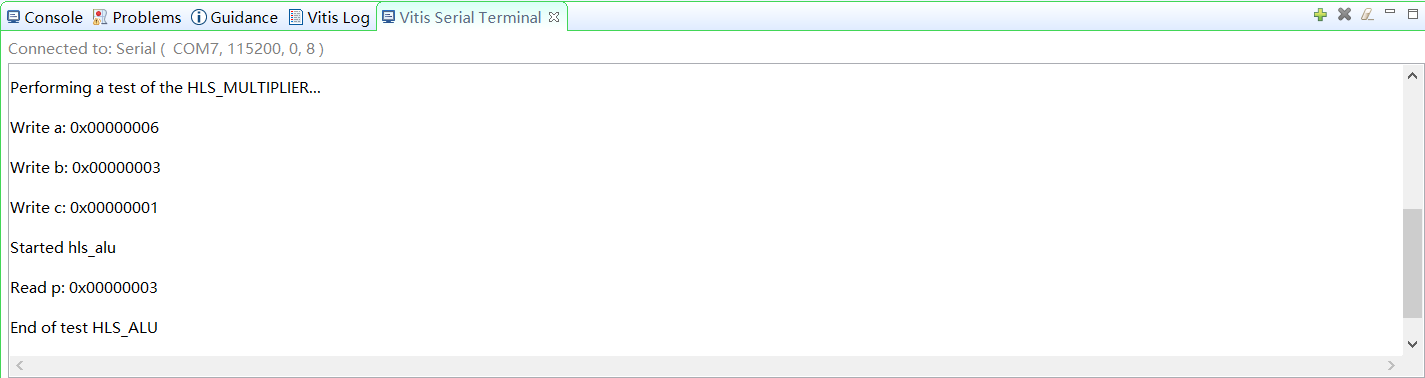
\includegraphics[width=1\textwidth]{7.png}
    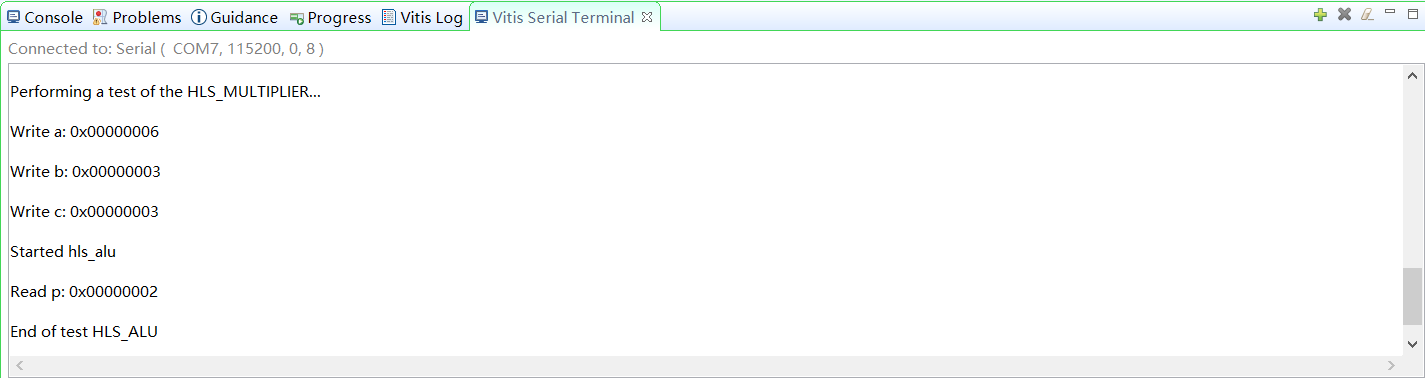
\includegraphics[width=1\textwidth]{8.png}
    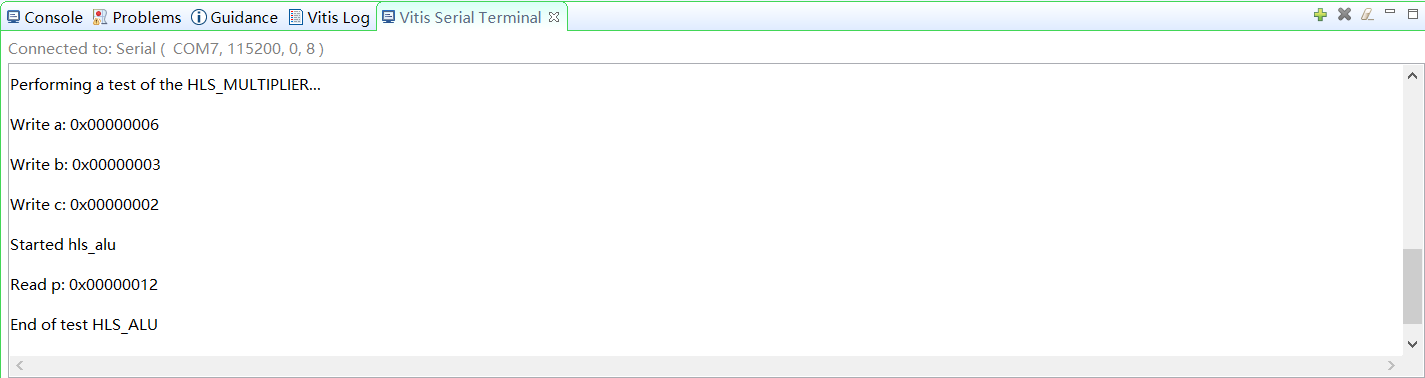
\includegraphics[width=1\textwidth]{9.png}
    \caption{SDK terminal printout of ALU.}
\end{figure}
For four arithmetic operations of ALU, we test them respectively. Code 0 indicates summation, which is 6+3=0. Code 1 indicates subtraction, which is 6-3=3. Code 2 indicates multiplication, which is 6*3=18=0x12. Code 2 indicates division, which is 6/3=2. 
\section{Programming the FPGA and Booting Software from the SD card}
\begin{figure}[H]
    \centering
    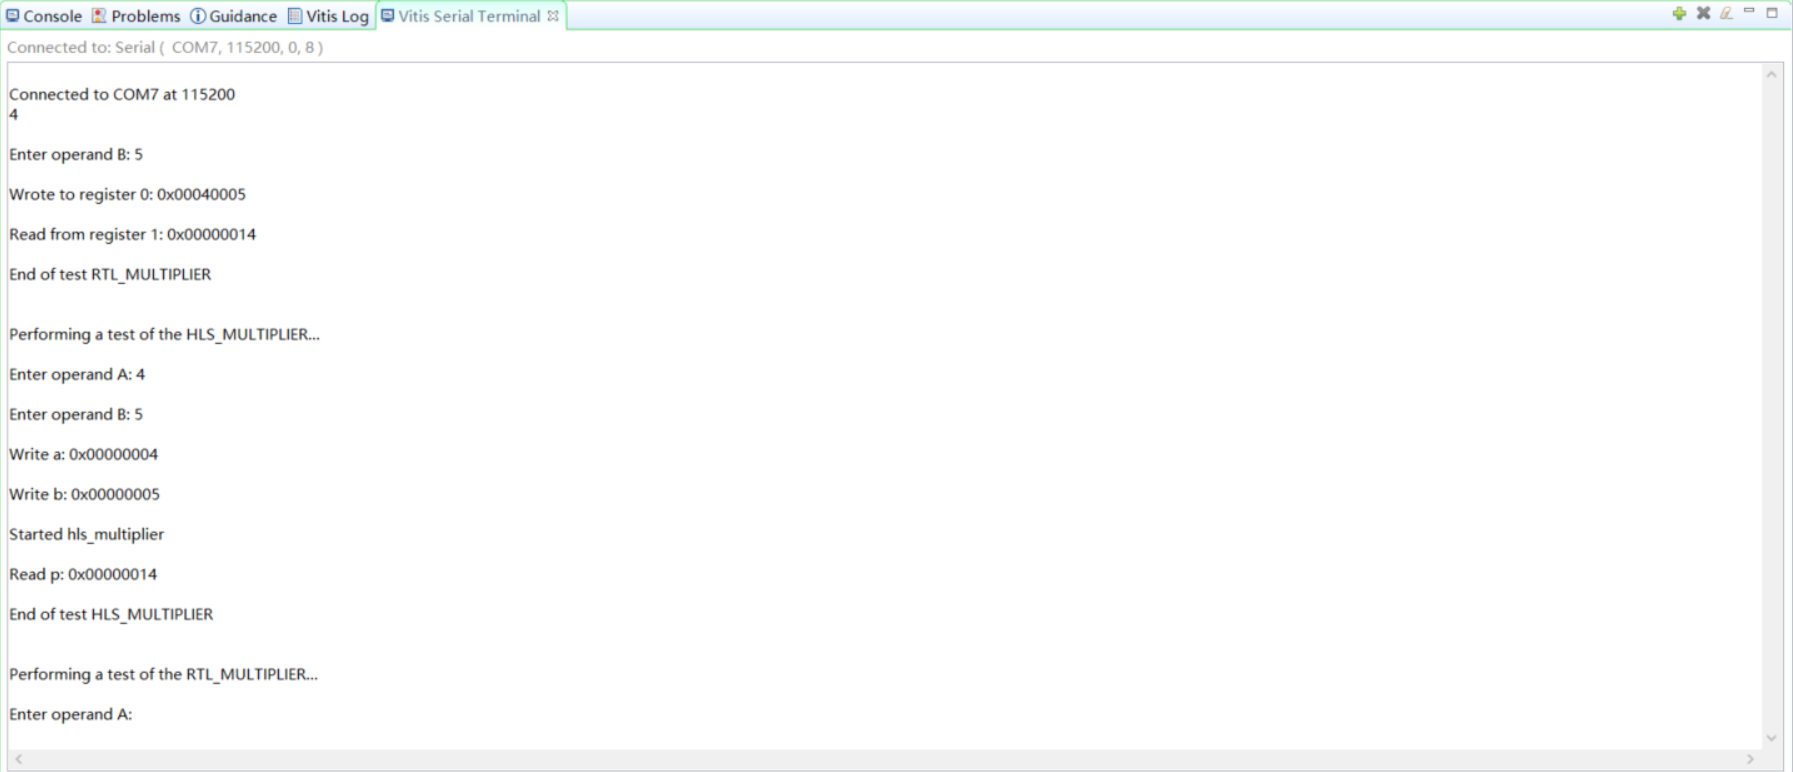
\includegraphics[width=1\textwidth]{10.png}
    \caption{The screenshot from the SDK terminal or PUTTY terminal.}
\end{figure}
\section{Programming Python on Arty Z7-20}
\begin{figure}[H]
    \centering
    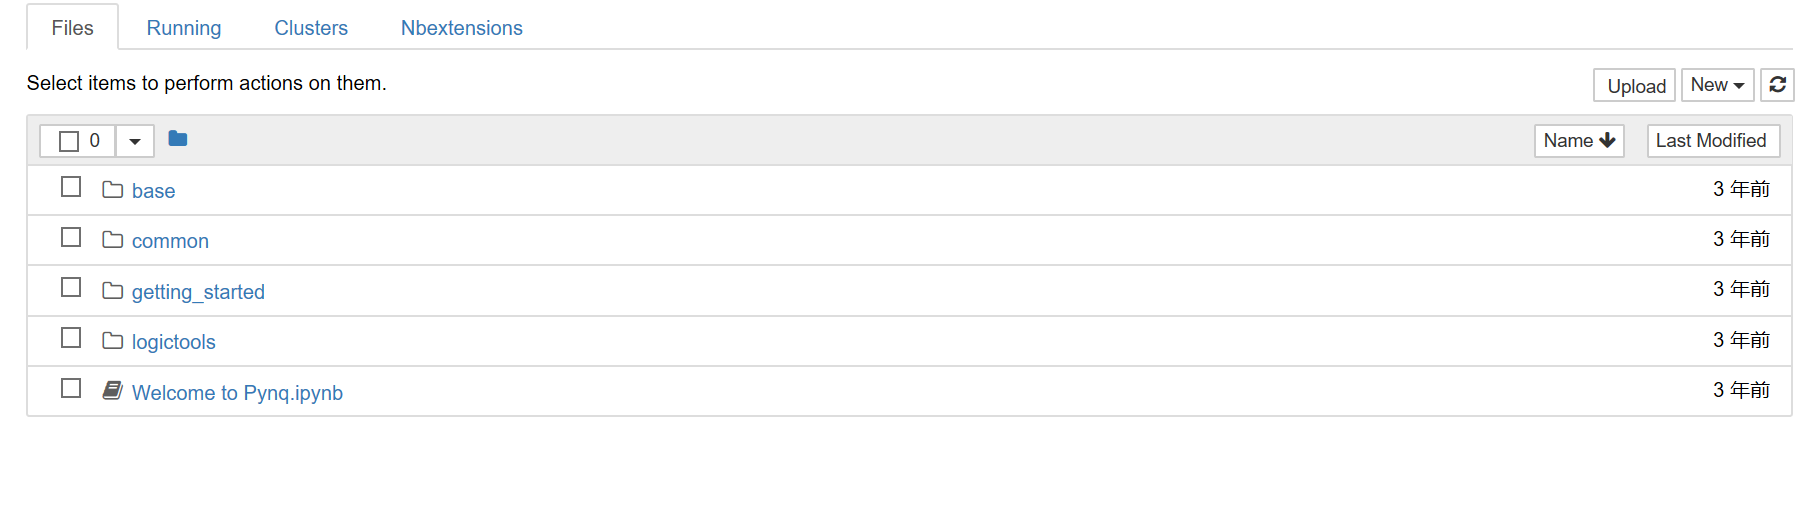
\includegraphics[width=1\textwidth]{11.png}
    \caption{The screenshot of the Jupyter notebook.}
\end{figure}
\section{Questions}
\begin{enumerate}
    \item What was the resource utilization of the rtl implementation vs. HLS implementation? If they are different, can you guess why there are differences?
    
    From previous results of RTL and HLS multiplier and divider in part 2, we find that RTL and HLS modules use different amount of building blocks on FPGA. Generally, the RTL implementation should be more compact comparing to HLS implementation. For instance of multiplier in Figure 1, the RTL implementation covers smaller area compared to HLS implementation. The reason is we can specific RTL hardware details and RTL module is logically optimized. However, for HLS implementation, there might be some redundant circuit elements. 
    
    Nevertheless, from our utilization report of RTL and HLS divider, we notice that HLS divider in fact consumes less recourse, which probably because our RTL implementation is not logically optimized enough. Besides, the high-level synthesis process itself also carries out some optimizations.
    \item Imagine that you have to create an IP block implementing 10 different sorting algorithms. Would you rather use a hardware description language or High-level Synthesis? Why?
    
    We would use high-level synthsis rather than hardware description language. The reason is that to implement an IP block with 10 different sorting algorithms manually by hardware description language is very complex and costs a lot of time on hardware logic, however, using high-level synthesis, it is much easier, and we can focus on implementing sorting algorithms themselves rather than hardware logic.
    \item Read more about PYNQ, and answer the following questions.
    \begin{enumerate}
    \item What is a Jupyter notebook? Why do we use it?\\
    Jupyter notebook is a platform which support Python and relating numerous packages we can easily dowload and use. It use blocks to execute codes step by step. Because we need to implement Pynq designs and Jupyter notebook can have a nice interface with the Arty-7z board through Ethernet connection to PC.
    \item What are overlays? What are the benefits of using overlays?\\
    Overlays are hardware designs made by hardware engineers for software engineers to use. Overlays are just like package in software programming, it can be used efficiently in other software design without having any knowledge about the hardware. It can be used to accelerate software or support the hardware platform for certain software. Convenience and modularity is the most benefit.
    \item Please list available overlays on the Arty-Z7 board.\\
    On the Arty-Z7, it supports BaseOverlay and Logictools Overlay. Also users can custom their own overlays.
    \item Comparing part 2 where you design with C/C++ vs. part 4 (PYNQ framework with python), what are the major differences?\\
    Design in C/C++ can accomplish more complicated and advanced function and it is more extensible. Besides, design with C/C++ is mature. In contrast, Pynq can take full advantage of package written in python and FPGA, which can shorten the design period and make it easier for design.
    \end{enumerate}
\end{enumerate}
\end{document}
